\fontfamily{ptm}\selectfont
\chapter{Result Analysis}
\section{Testing}
Table \ref{test1} gives details of validation.


\begin{table}[h!]
  \begin{center}
    \caption{Test Case Validation}
    \label{test1}
    \begin{tabular}{|p{1cm}|p{4cm}|p{4cm}|p{4cm}|}
    \hline
      \textbf{Test Case No.} & \textbf{Input} & \textbf{Expected 
Output} & \textbf{Actual Output}\\

\hline
     1 & User registers & Successful registration & Successful registration \\
\hline
2 & Meal listing creation & Listing created & Listing created \\
\hline
3 & Meal browsing & Available meals listed & Available meals listed \\
\hline
4 & Meal request & Request submitted & Request submitted \\
\hline
5 & NGO booking & Meal booked & Meal booked \\
\hline
6 & User confirmation & Confirmation received & Confirmation received \\
\hline
7 & User logout & Logout successful & Logout successful \\
\hline
8 & Account type adjustment & Account type updated & Account type updated \\
\hline
     \end{tabular}
  \end{center}
\end{table}
\begin{figure}[H]
     \centering
     \begin{subfigure}[b]{0.3\textwidth}
         \centering
         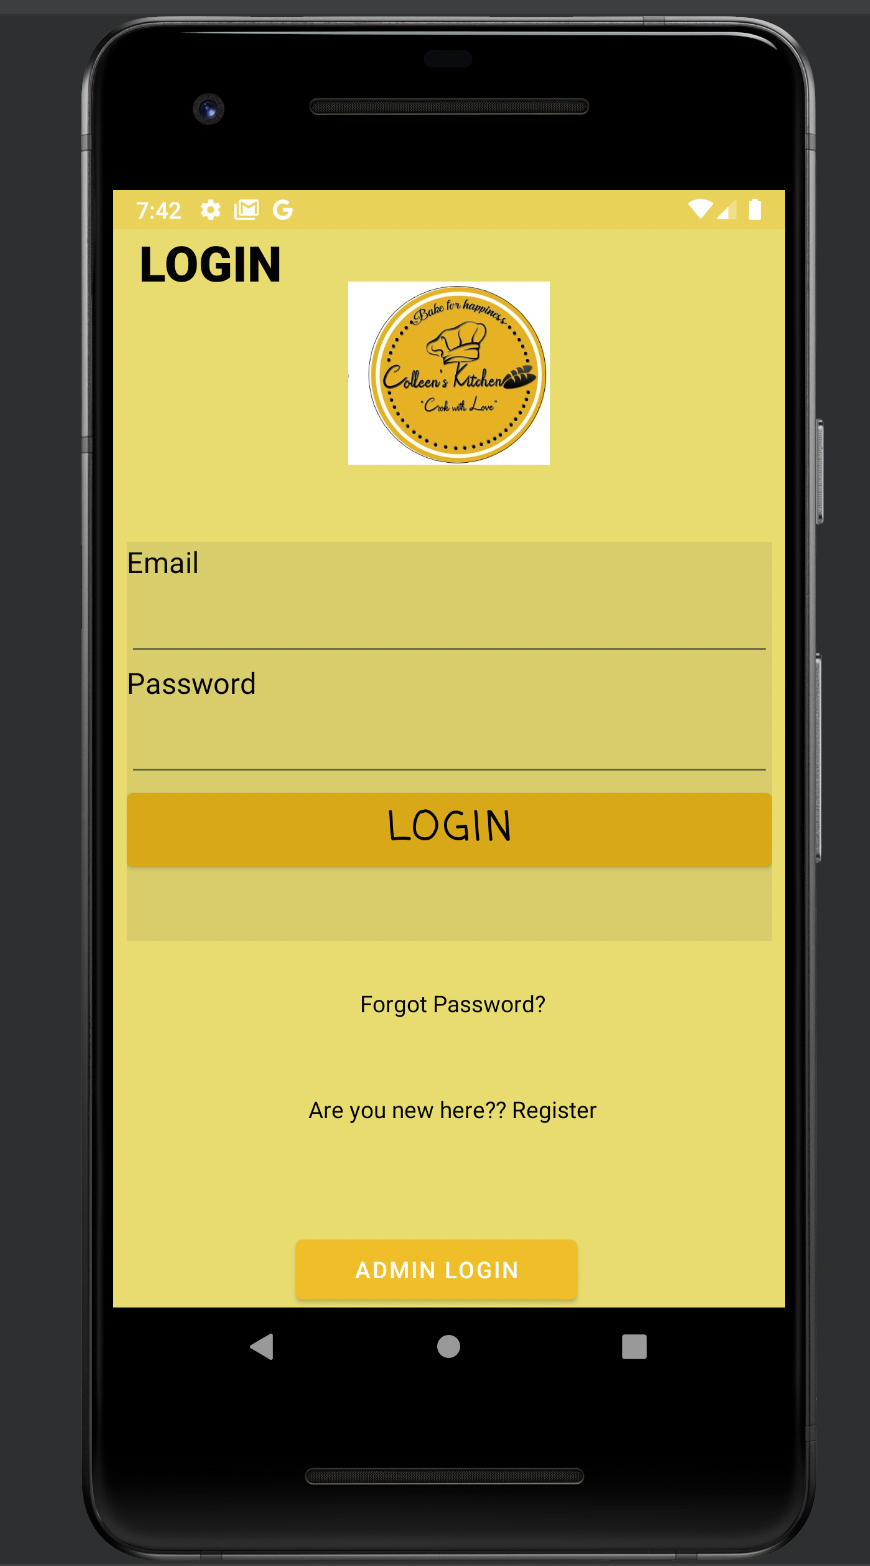
\includegraphics[width=\textwidth]{m1}
         \caption{Allows User To Login}
         \label{first disp}
     \end{subfigure}
     \hfill
     \begin{subfigure}[b]{0.3\textwidth}
         \centering
         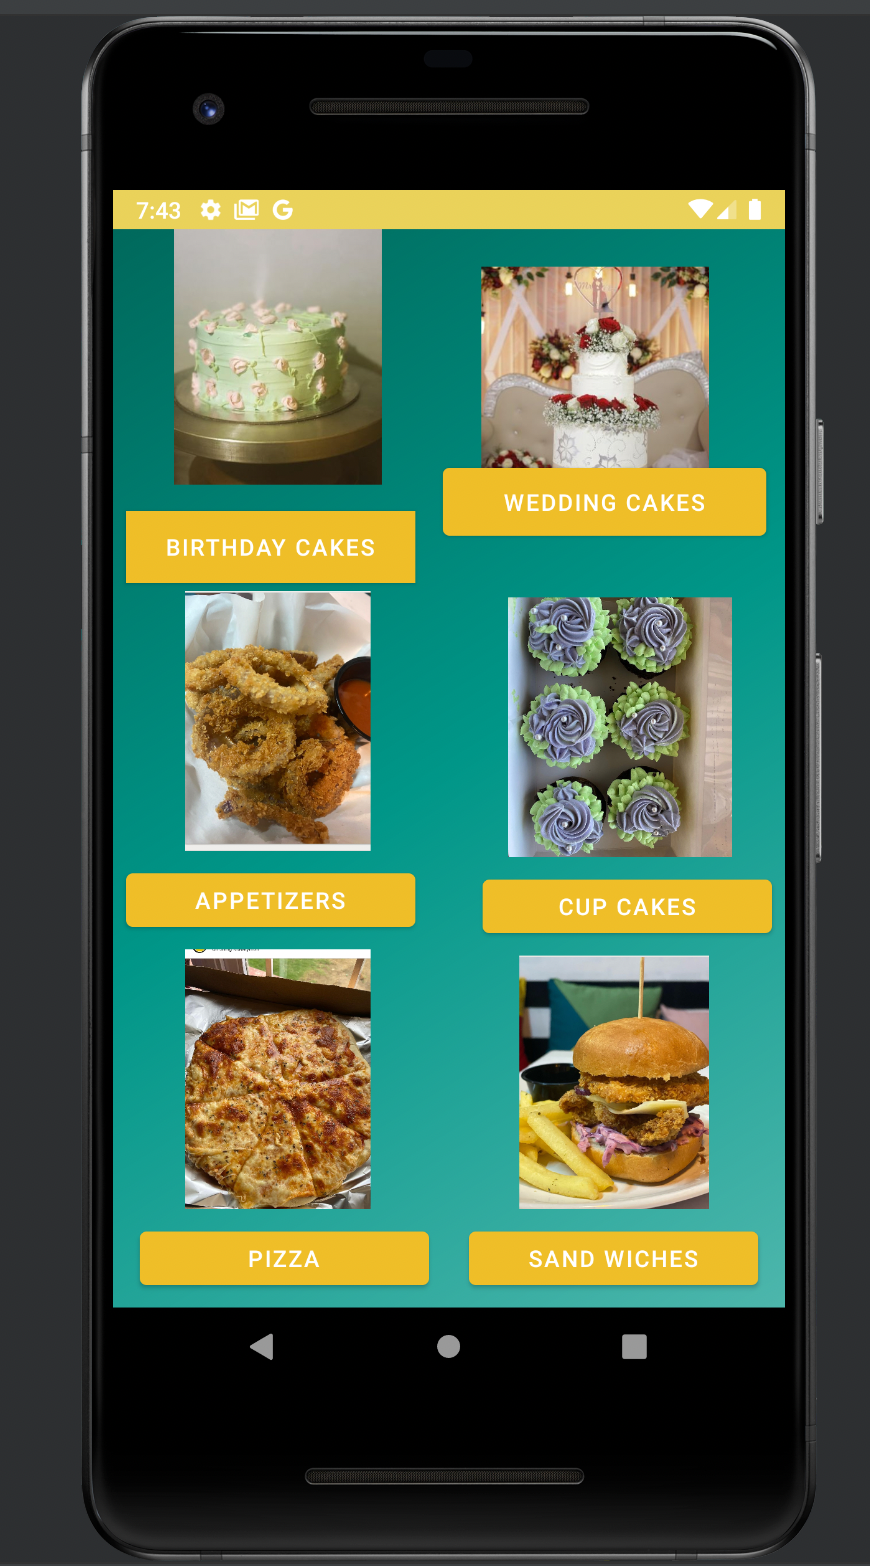
\includegraphics[width=\textwidth]{m2}
         \caption{Products in Category wise}
         \label{sec disp}
     \end{subfigure}
     \hfill
     \begin{subfigure}[b]{0.3\textwidth}
         \centering
         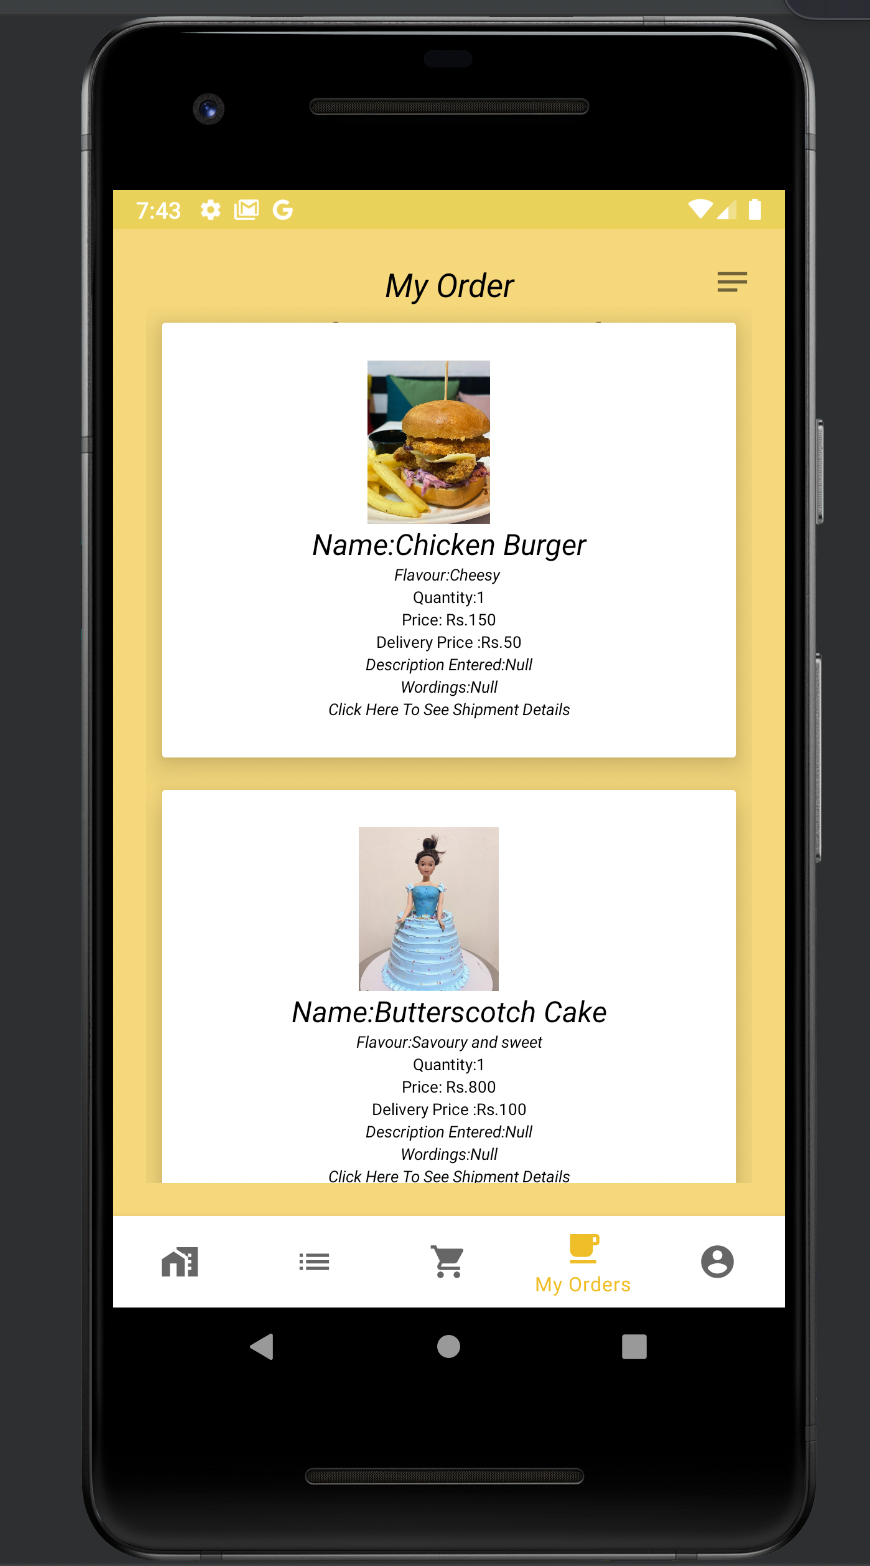
\includegraphics[width=\textwidth]{m3}
         \caption{Order Successfully Placed}
         \label{third disp}
     \end{subfigure}
     \hfill
     \\
     \vspace{20pt}
     \begin{subfigure}[b]{0.3\textwidth}
         \centering
         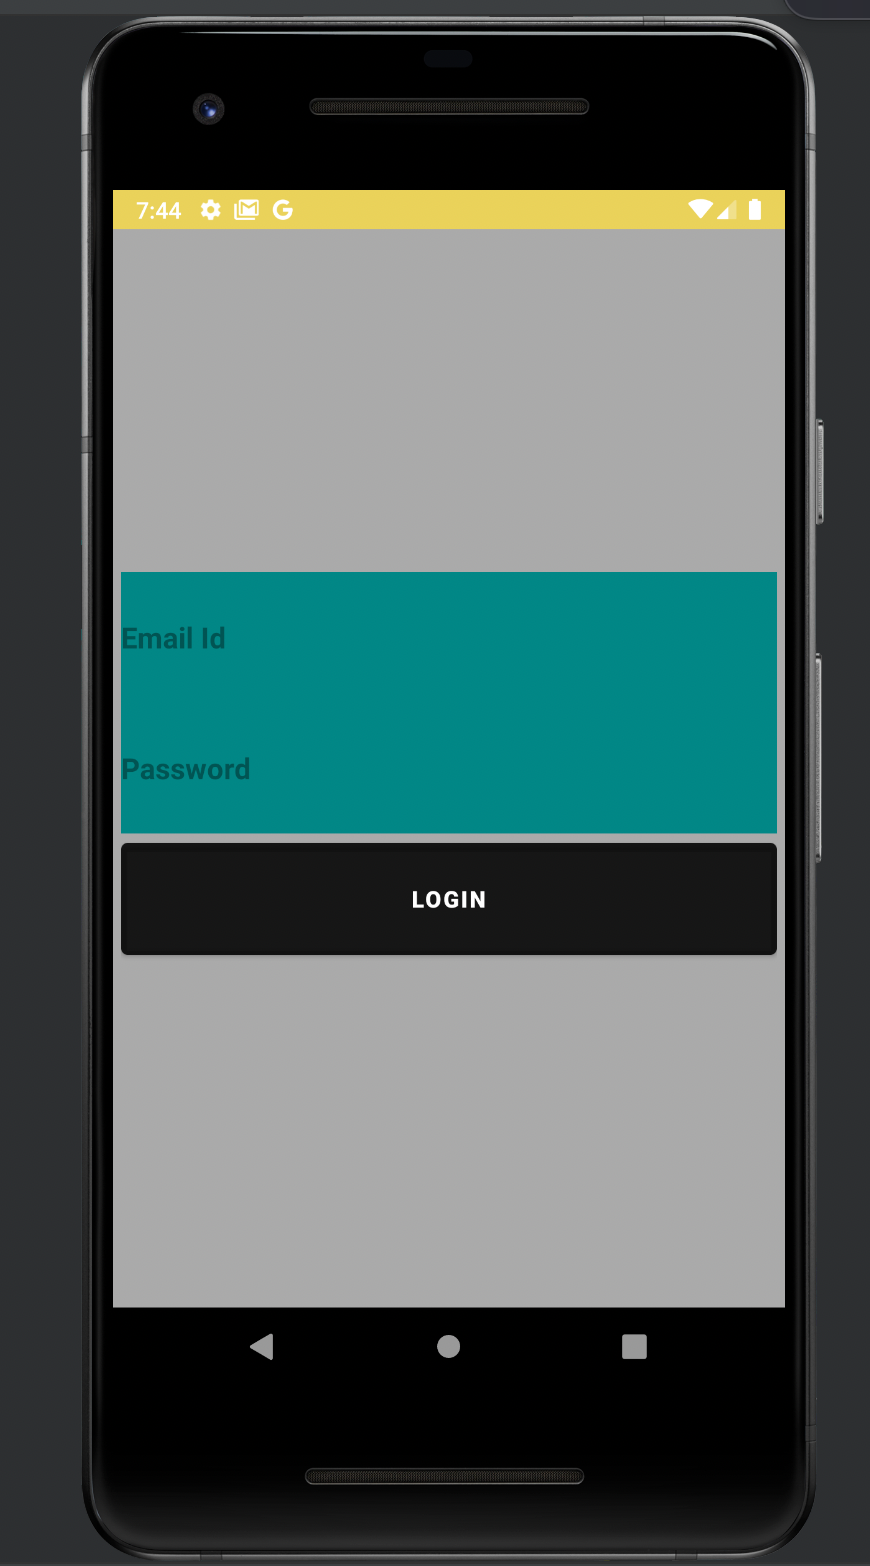
\includegraphics[width=\textwidth]{m4}
         \caption{Allow Admin To Login}
         \label{third disp}
     \end{subfigure}
     \hfill
     \begin{subfigure}[b]{0.3\textwidth}
         \centering
         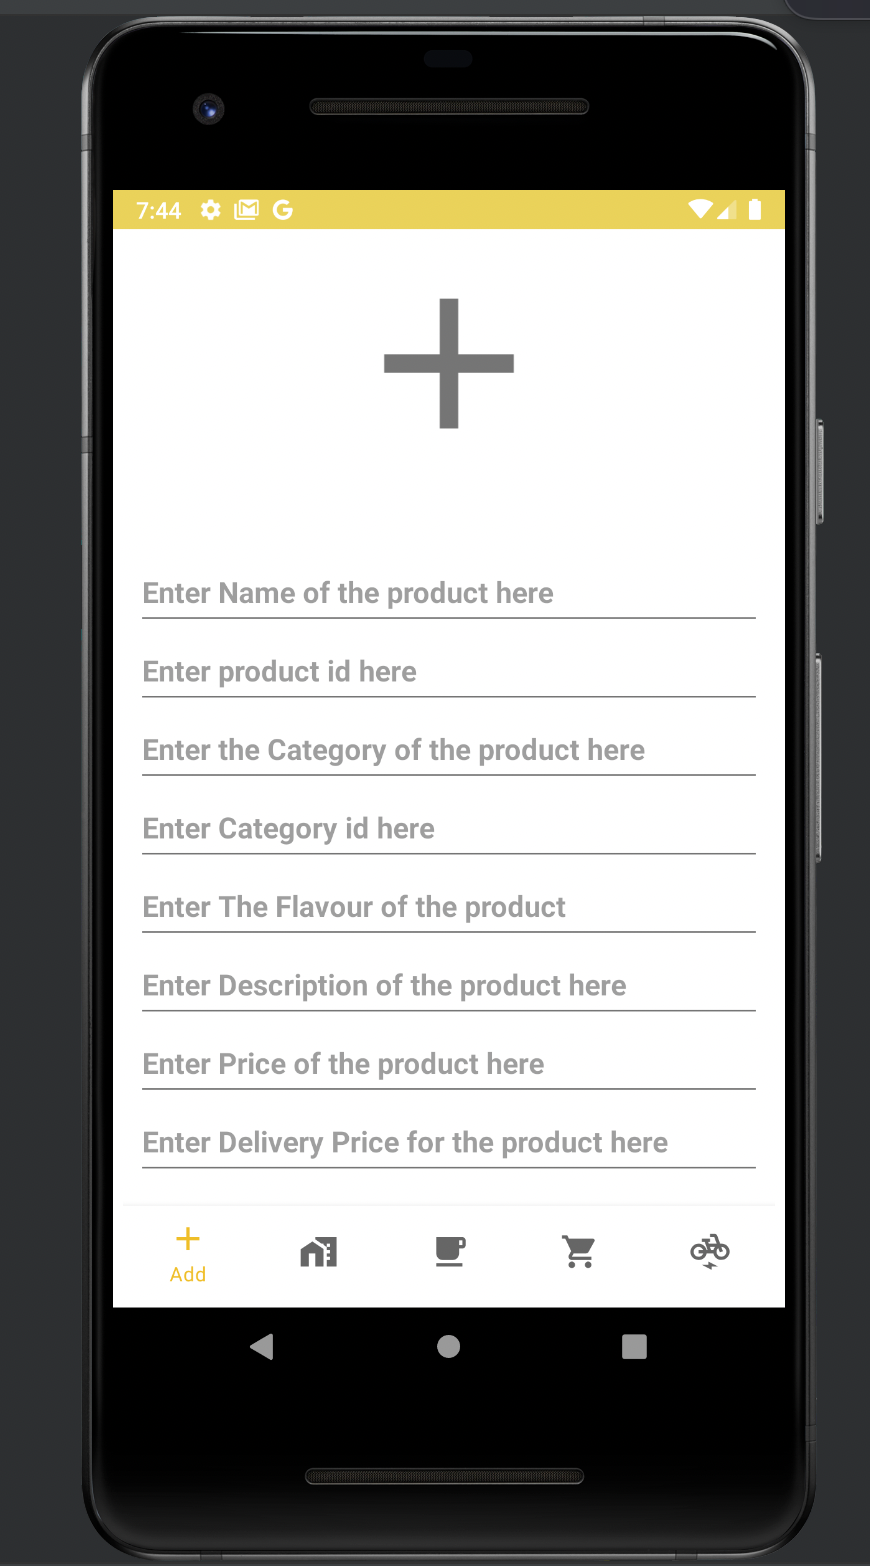
\includegraphics[width=\textwidth]{m5}
         \caption{Admin Adding Products}
         \label{third disp}
     \end{subfigure}
     \hfill
     \begin{subfigure}[b]{0.3\textwidth}
         \centering
         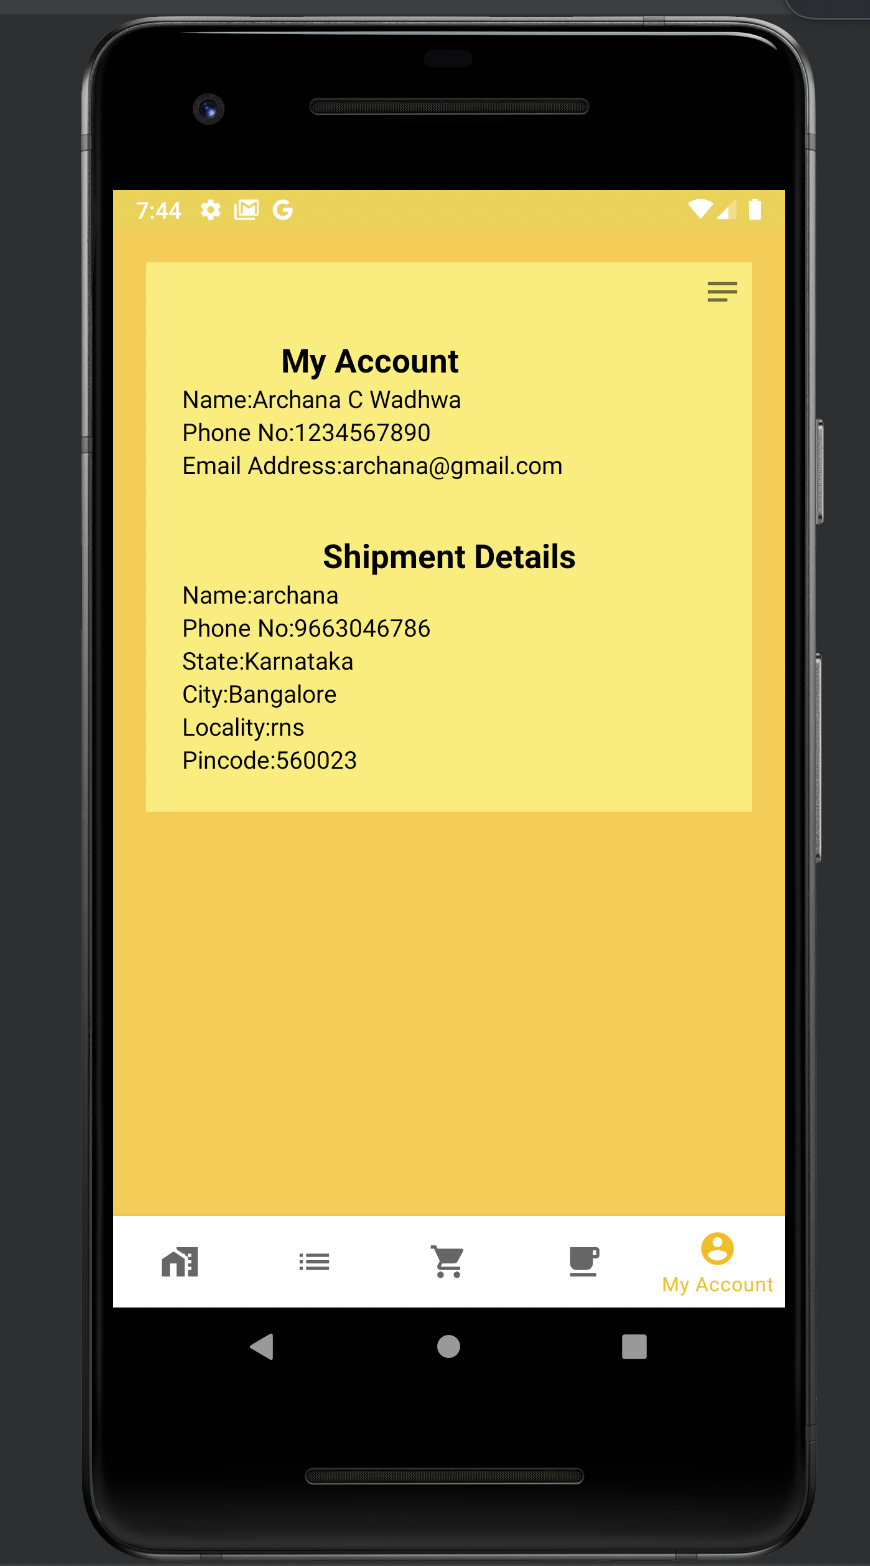
\includegraphics[width=\textwidth]{m6}
         \caption{Account \& Shipment Details }
         \label{third disp}
     \end{subfigure}
        \vspace{10pt}
        \caption{ Output for test cases of Meal Mingle.}
        \label{fig3}
\end{figure}

\chapter{Conclusion}
 In conclusion, the MealMingle project offers a comprehensive and user-friendly solution to address the pressing issues of food waste and food insecurity. By providing a centralized platform that facilitates coordination and communication between surplus food providers, individuals in need, hotels, restaurants, and NGOs, MealMingle aims to overcome the limitations of existing systems. The project's focus on scalability, technological integration, and data-driven decision-making ensures a more efficient and impactful approach.

Through MealMingle, individuals can easily share their excess meals, hotels and restaurants can contribute surplus food, and NGOs can directly book meals for those facing food insecurity. The app's features, such as meal browsing, direct booking, and volunteer opportunities, promote collaboration, reduce food waste, and foster a sense of community. By leveraging technology and community participation, MealMingle not only addresses immediate hunger relief but also encourages sustainable food consumption practices.

With its potential for wide-scale adoption, MealMingle has the power to create a meaningful social impact by bridging the gap between surplus food and those in need. By utilizing the platform, individuals, hotels, restaurants, and NGOs can actively contribute to reducing food waste and alleviating food insecurity within their communities. Together, we can create a stronger, more compassionate society where no one goes hungry.

In conclusion, MealMingle presents a promising solution to combat food waste and food insecurity, paving the way for a more sustainable and equitable future.